%----------------------------------------------------------------------------------------
%	PACKAGES AND OTHER DOCUMENT CONFIGURATIONS
%----------------------------------------------------------------------------------------
\documentclass[a4paper,11pt]{article}

%Include Packages
%----------------------------------------------------
\usepackage{../Header/KaTeX_LabReport}
\usepackage{lipsum}
% Note: 
% The input command is equivalent to copy-paste the content of the file
% into the current file.

\renewcommand{\thesection}{\Roman{section}} 
\titleformat{\section}[display]%command shape
    {\Huge}%format
    {
        \newpage
        \setlength\fboxsep{0pt}
        \color{gray} \fontsize{20}{5}\selectfont\chaptername\ \thesection
    }%label
    {0pt}{}{}
\titlespacing*{\section}{0pt}{0pt}{20pt}
\renewcommand{\thesubsection}{\thesection: \Roman{subsection}}
\renewcommand{\thesubsubsection}{\thesubsection. \roman{subsubsection}}
\renewcommand{\thesubsection}{\Roman{subsection}}
\titleformat{\subsection}
    {\bfseries\Large}%format
    {\huge\textnormal{\thesubsection}}%label
    {12pt}{}{}

\usepackage{sectsty}
    \sectionfont{\LARGE}
    \subsectionfont{\large}
    \subsubsectionfont{\large}
    \paragraphfont{\large}
\usepackage{titletoc}
    \titlecontents{}[1em]{\addvspace{1pc}\bfseries}      {\contentslabel{3em}}{}
    {\titlerule*[0.3pc]{.}\contentspage}

\usepackage{tocloft}% http://ctan.org/pkg/tocloft
\setlength\cftsecnumwidth{6em}

\renewcommand{\thesubsubsection}{\thesubsection: \roman{subsubsection}}
\titlespacing{\subsubsection}{0pt}{15pt}{5pt}

%Hyperlink Setting
%----------------------------------------------------
\hypersetup{hidelinks,
	colorlinks=true,
	allcolors=black,
	pdfstartview=Fit,
	breaklinks=true
}

% \includeonly{
%     Experiment_01/Lab1_Main,
%     Experiment_02/Lab2_Main,
%     Experiment_07/Lab7_Main,
% }

\begin{document}
%----------------------------------------------------------------------------------------
%	FRONT MATTER
%----------------------------------------------------------------------------------------
% Cover
\thispagestyle{empty}
\begin{titlepage}
    % Warning Filter
    \WarningFilter[latex]{latexfont}{Some font shapes}
    \WarningFilter[latex]{tex}{Underfull \hbox}
    \ActivateWarningFilters[latex]

	%\hspace{0.05\textheight} % Whitespace between the vertical line and title page text
    \parbox{1\textwidth}{ % Paragraph box for holding the title page text, adjust the width to move the title page left or right on the page
		{\Huge\bfseries EIE420 Assignment II \\[0.15\baselineskip] 
        Gray Scale Histrogram}\\[0.15\baselineskip] % Title
		\rule{1\textwidth}{1pt} % Vertical line
        {\Large\textit{Report of EIE420, Digital Image Processing Assignment}}
        \newline
    }
    \parbox{1\textwidth}{
        \vspace{1\baselineskip}
        \large
        Source Code of this assignment could be found at:\newline
        \url{https://github.com/ZeppelinSCB/EIE420-Digital_Image_Processing}
        \newline
    }
    \vspace{100pt} % Whitespace between the title block and the publisher
    \parbox{1\textwidth}{
        {\large by}\\[1.5\baselineskip]
        {\rule[1pt]{200pt}{1pt}} \\[1.25pt]
        {\huge\textsc{Pengrui K. Tong}
            %\begin{CJK*}{UTF8}{bsmi}\Large (湯鵬睿)\end{CJK*}
            }\\
        {\large{Student No: 1220031811}} \\
        \large from EIE420 D1, \newline
        Faculty of Innovation Engeneering, \newline
        Universidade de Ciência e Tecnologia de Macau
    }
		

    \vspace*{\fill}
		Apr 6, 2025 \newline 
        (Coloane, Macao, SAR)
        \vspace{0.7\baselineskip}\newline
        %
\includegraphics[width = 40mm]{MUIT_BlueGold.png}\newline
        
\includegraphics[width = 40mm]{../Header/MUIT_origin.png}\par
        {\small Cover Design by Karl Tong}\\[0.25pt]
        {\small This report is a part of the result for}
        {\small EIE420~Digital~Image~Processing in U.C.T.M}\\[0.25pt]
        {\small \copyright 2025 Pengrui Tong}
\end{titlepage}
\blankpage

% Table of Contents
\tableofcontents
\blankpage
\section{Bacgkground}
Image scaling with interpolation is a common task in image processing. It involves resizing an image while maintaining its quality and details as much as possible. Modern methods leverage machine learning and deep learning techniques to produce sharp and clear images.

\section{Problem Statement}
This experiment aims to implement a MATLAB function, $Scaling_K$, capable of scaling images to any specified size using bilinear or nearest-neighbor interpolation. The challenge lies not only in correctly applying these interpolation methods but also in ensuring the function can accurately scale very small pixel art, which demands careful handling the edges of the image where the result pixel map to places of he original image that didn't have neighboring pixels as expected.

\section{Procedure}
\subsection{Principle of the Algorithm}
In both algorithm, we use the backward mapping method to find the pixel value of the new image. The backward mapping method is we traversal all the pixels in the new image, and for each pixel, we find the corresponding pixel in the original image. And we use one of the interpolation methods to decide the pixel value of the new image. \\
Let \( I \) be the source image and \( I' \) the scaled image. For target coordinates \((x', y')\), we find its cooresponding coordinates in the source image \((x, y)\) using the following equations:
\begin{equation}
    x = \frac{x'}{scale}, \quad y = \frac{y'}{scale},
\end{equation}
where $scale$ are the scaling factor. And we find the nearest integer coordinates in the source image:

\subsubsection{Nearest-Neighbor Interpolation}
    For pixel $I'(x', y')$ in the result image, let its value equals to the nearest pixel in the source image:
    \begin{equation}
        I'(x', y') = 
            I\left(roud(x + 0.5), round( y + 0.5 )\right)
        \label{eq:nn}
    \end{equation}
    Note we add 0.5 to the coordinates before flooring so the starting pixel of rows and columns can map to the pixel with index 1 correctly.

\subsubsection{Bilinear Interpolation}
    For pixel $I'(x', y')$ that maps to the pixel $I(x, y)$. The interpolated value combines four neighbors using distance-weighted averaging:
    \begin{equation}
        I'(x', y') = (1 - dx)(1 - dy)I_{x,y} + dx(1 - dy)I_{x+1,j} + (1 - dx)dyI_{i,y+1} + dx \cdot dy \cdot I_{x+1,y+1}.
        \label{eq:bilinear}
    \end{equation}
    This smooths pixel transitions better than nearest-neighbor.
    

\subsection{Design of the Algorithm}
\subsubsection{The Image Scaling Function}
One issue I encountered is index out of bound error for some specfic scale. And I slove the problem by using the \texttt{floor} function to round down the dimensions of the scaled image. Compairs to \texttt{round}, this ensures that the output pixel won't map to the edge of the original image.\\
\textbf{Input:} 
\begin{itemize}
    \item \textbf{imIn} (Numeric Matrix):\\
        Input image matrix (grayscale or RGB). Dimensions: 2 or 3
    \item \textbf{scale} (Positive Scalar):\\
        Scaling factor. Must be $>0$. Values $>1$ enlarge the image; $<1$ shrink it.
    \item \textbf{method} (nearest | bilinear):\\
        \texttt{ScaleMethod.nearest} (0) for nearest-neighbor or\\
        \texttt{ScaleMethod.bilinear} (1).
\end{itemize}
\textbf{Output:}
\begin{itemize}
    \item \textbf{imScaled} (uint8 Matrix):\\
        Scaled output image. 
        Dimensions are rounded down using \texttt{floor} to avoid indexing errors \\
        (e.g., initial $5 \times 5$ scaled by 2.5 becomes $12 \times 12$).
\end{itemize}
\textbf{Algorithm:}
\begin{enumerate}
\item \textbf{Parameter Validation}
    \begin{enumerate}
        \item Verify \texttt{scale} $>0$; else, throw error.
        \item Check if \texttt{method} is valid (\texttt{nearest} or \texttt{bilinear}). Invalid methods trigger an error.
        \item Validate image dimensions (2D or 3D); unsupported formats throw errors.
    \end{enumerate}
\item \textbf{Initialize Output Image (\texttt{imOut})}
    \begin{enumerate}
        \item Compute scaled dimensions with \texttt{floor(dimensions * scale)} to avoid floating-point indexing errors.
        \item Allocate \texttt{imOut} as a zero-filled \texttt{uint8} matrix matching the scaled size.
    \end{enumerate}
\item \textbf{Execute Interpolation}
    \begin{enumerate}
        \item For \texttt{nearest}, call \texttt{NN\_K} to apply nearest-neighbor interpolation.
        \item For \texttt{bilinear}, call \texttt{DL\_K} to compute bilinear interpolation.
    \end{enumerate}
\end{enumerate}

\subsubsection{The Nearest-Neighbor Interpolation Function}
\begin{figure}[H]
    \centering
    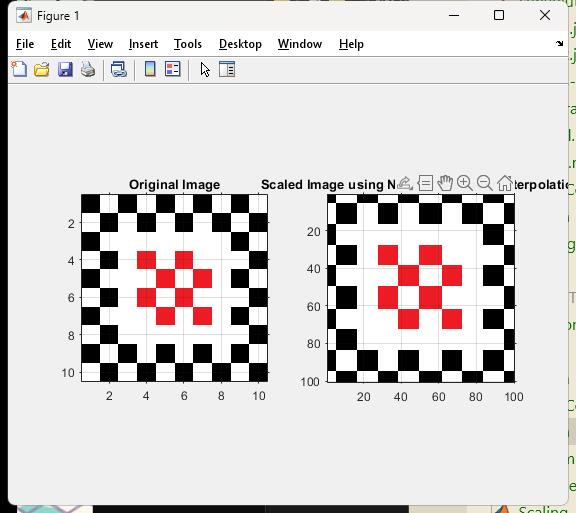
\includegraphics[width=0.8\linewidth]{Don't support Pixel image.jpg}
    \caption{If don't add 0.5 before rounding, the result won't be ideal}
    \label{pic:Issue2}
\end{figure}
When rouding for the coordinates, I add 0.5 to the coordinates before flooring so the starting pixel of rows and columns can map to the pixel with index 1 correctly, and will provides an accurate result even for image with extremely small size.\\
\textbf{Input:}
\begin{itemize}
    \item \textbf{imIn} (uint8[][][]):\\
        Input image matrix with Dimensionsof three.
    \item \textbf{imOut} (uint8[][][]):\\
        Preallocated output matrix initialized with zeros.
    \item \textbf{scale} (float):\\
        Scaling factor.
\end{itemize}

\textbf{Output:}
\begin{itemize}
    \item \textbf{imScaled} (uint8[][][]):\\
        Scaled image using nearest-neighbor interpolation.
\end{itemize}

\textbf{Algorithm:}
\begin{enumerate}
\item \textbf{Enlarge Image to Avoid Index Overflow}
    \begin{enumerate}
        \item Extend \texttt{imIn} by replicating its last row and column into \texttt{imEnlarged}. Ensures valid indices when mapping edge pixels.
    \end{enumerate}
\item \textbf{Coordinate Mapping \& Pixel Assignment}
    \begin{enumerate}
        \item For each output pixel \((row, col)\):
            Compute corresponding input coordinates using equation \ref{eq:nn}\\
            Assign nearest-neighbor value from enlarged source image \texttt{imEnlarged(rOrg, cOrg)} to \texttt{imScaled(row, col)}.\\
    \end{enumerate}
\end{enumerate}


\subsubsection{The Image Scaling Function (Bilinear Interpolation)}
\textbf{Input:}
\begin{itemize}
    \item \textbf{imIn} (Numeric Matrix):\\
        Input image matrix (grayscale/RGB). Dimensions: 2 (height $\times$ width) or 3 (height $\times$ width $\times$ channels).
    \item \textbf{imOut} (uint8 Matrix):\\
        Preallocated output matrix initialized with zeros. Size matches scaled dimensions derived from \texttt{floor}.
    \item \textbf{scale} (Positive Scalar):\\
        Scaling factor: $a > 1$ enlarges, $a < 1$ shrinks. Coordinates mapped inversely: output pixels trace back to padded input space.
\end{itemize}

\textbf{Output:}
\begin{itemize}
    \item \textbf{imScaled} (uint8 Matrix):\\
        Scaled image via bilinear interpolation. Initialized as a zeros matrix matching \texttt{imOut}'s dimensions.
\end{itemize}

\textbf{Algorithm:}
\begin{enumerate}
\item \textbf{Replicated Padding (Edge Handling)}
    Pad \textbf{imIn} with replicated borders:\\
              - Add first row to the top and last row to the bottom.
              - Add first column to the left and last column to the right.
              Creates a 1-pixel buffer to avoid index errors during interpolation.
\item \textbf{Coordinate Mapping \& Bilinear Blending}
    For each output pixel \((row, col)\):
            \begin{itemize}
                \item Compute input coordinates in padded space (see Equation~\ref{}).
                \item Calculate the pixel value of each channels using Equation \ref{eq:bilinear}.
            \end{itemize}
\end{enumerate}


\section{Source Code}
\subsection{Code of Scaling Function}
\lstset{language = Matlab}
\begin{lstlisting}[basicstyle=\tiny]
    %This function provides a image scaling algorithm.
    % TODO: implement support for gray scale image
    function [imScaled] = Scaling_K(imIn, scale, method)
        % Validate parameters
        dimensions = size(imIn);
        if scale <= 0
            error('Scale factor must be greater than 0.');
        end
        if method ~= ScaleMethod.nearest && method ~= ScaleMethod.bilinear
            error('Invalid method. Use 0 for Nearest Neighbor or 1 for Bilinear.');
        end
        % Note to use floor to avoid rounding error caused by floating point then cause index out of bound
        switch length(dimensions)
            case 2 
                imOut = zeros(floor(dimensions(1)*scale), floor(dimensions(2)*scale), "uint8");
            case 3
                imOut = zeros(floor(dimensions(1)*scale), floor(dimensions(2)*scale), dimensions(3), "uint8");
            otherwise
                error('Unsupported image format. Must be matrix with dimension of 2 or 3.');
        end
        % Perform scaling
        switch method
            case ScaleMethod.nearest
                imScaled = NN_K(imIn, imOut, scale);
            case ScaleMethod.bilinear
                imScaled = DL_K(imIn, imOut, scale);
            otherwise
                error('Invalid method. Use 0 for Nearest Neighbor or 1 for Bilinear.');
        end
    end
\end{lstlisting}

\subsection{Code of Nearest-Neighbor Interpolation}
\lstset{language = Matlab}
    \begin{lstlisting}[basicstyle=\tiny]
    function [imScaled] = NN_K(imIn, imOut, scale)
        imEnlarged = [
            imIn;
            imIn(end,:,:)
        ];
        imEnlarged = [
            imEnlarged, imEnlarged(:,end,:);
        ];
        imScaled = ones(size(imOut), "uint8");
        for row = 1:size(imOut, 1)
            for col = 1:size(imOut, 2)
                rOrg = round((row)/scale+0.5); %shift 1 row down to avoid 0 index
                cOrg = round((col)/scale+0.5); %shift 1 column down to avoid 0 index
                imScaled(row, col,:) = imEnlarged(rOrg,cOrg,:);
            end
        end
    end
\end{lstlisting}

\subsection{Code of Nearest-Neighbor Interpolation}
\lstset{language = Matlab}
    \begin{lstlisting}[basicstyle=\tiny]
    function [imScaled] = DL_K(imIn, imOut, scale)
        imScaled = zeros(size(imOut), "uint8");
        imEnlarged = [
            imIn(1,:,:);
            imIn;
            imIn(end,:,:)
        ];
        imEnlarged = [
            imEnlarged(:,1,:), imEnlarged, imEnlarged(:,end,:);
        ];
        for row = 1:size(imOut, 1)
            for col = 1:size(imOut, 2)
                rOrg = 1+row/scale;
                cOrg = 1+col/scale;
                x = (1-mod(cOrg, 1));
                y = (1-mod(rOrg, 1));
                %NE
                pixNE = imEnlarged(floor(rOrg),floor(cOrg),:).*x.*y;
                pixNW = imEnlarged(floor(rOrg),floor(cOrg)+1,:).*(1-x).*(y);
                pixSE = imEnlarged(floor(rOrg)+1,floor(cOrg),:).*(x).*(1-y);
                pixSW = imEnlarged(floor(rOrg)+1,floor(cOrg)+1,:).*(1-x).*(1-y);
                imScaled(row, col,:) = pixNE + pixNW + pixSE + pixSW;
            end
        end
    end
\end{lstlisting}

\section{Discussion}

\subsection{Testing Program Output}
I tested the function with a custom 10x10 image, and scale random from 0 to 5. And this testing program helps me find serval errors in the code. \\
The first one is the index out of bound error for destination size with remainder grater than 0.5, and this is sloved by using the \texttt{floor} function to round down the dimensions of the scaled image. The second one is the image didn't scale properly for small scale image. This is caused by the way I treat the edge, and sloved by adding 0.5 to the coordinates before flooring so the starting pixel of rows and columns can map to the pixel with index 1 correctly.\\

\begin{figure}[H]
    \centering
    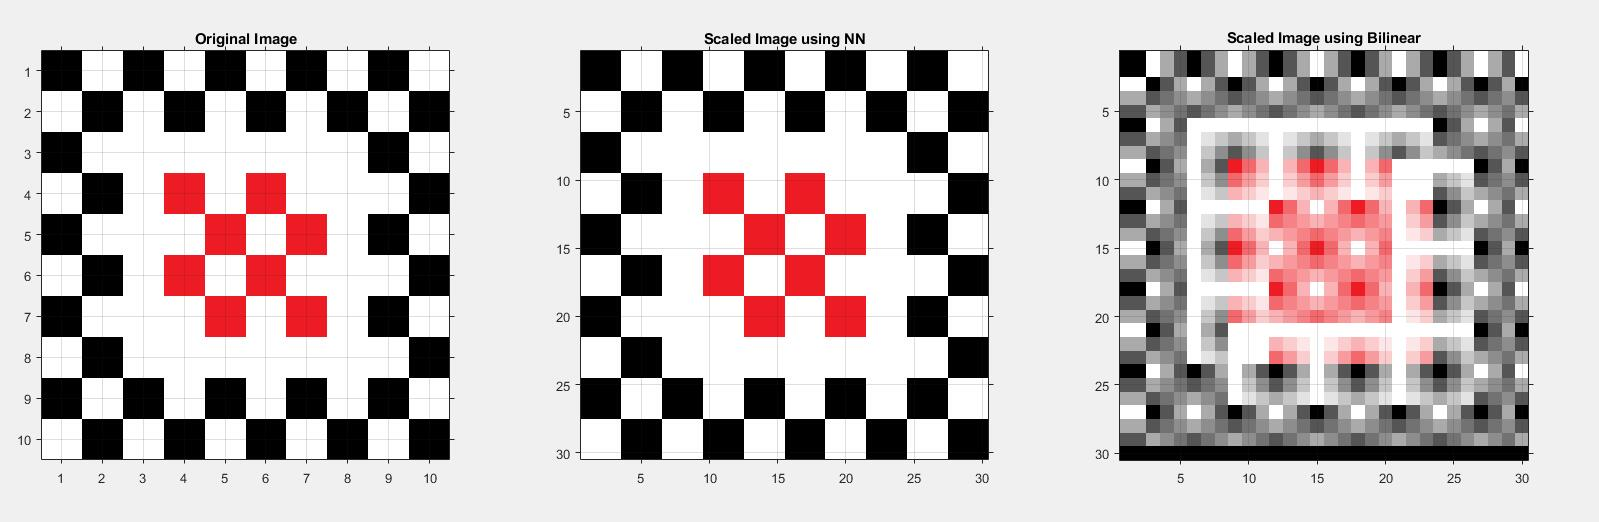
\includegraphics[width=0.8\linewidth]{FinalResult.jpg}
    \caption{Chessboard Tesing Image}
    \label{pic:Demo_1}
\end{figure}
After sloving the errors, my function can scale the image properly. The result is shown in figure \ref{pic:Demo_1}.\\

To compair the two methods, I use some real images to both scale up and down some images, the result is shown in figure \ref{pic:Demo_2} and figure \ref{pic:Demo_3} respectivly, with the , left: original image, middle, nearest neighbor right: bilinear.\\

\begin{figure}[H]
    \centering
    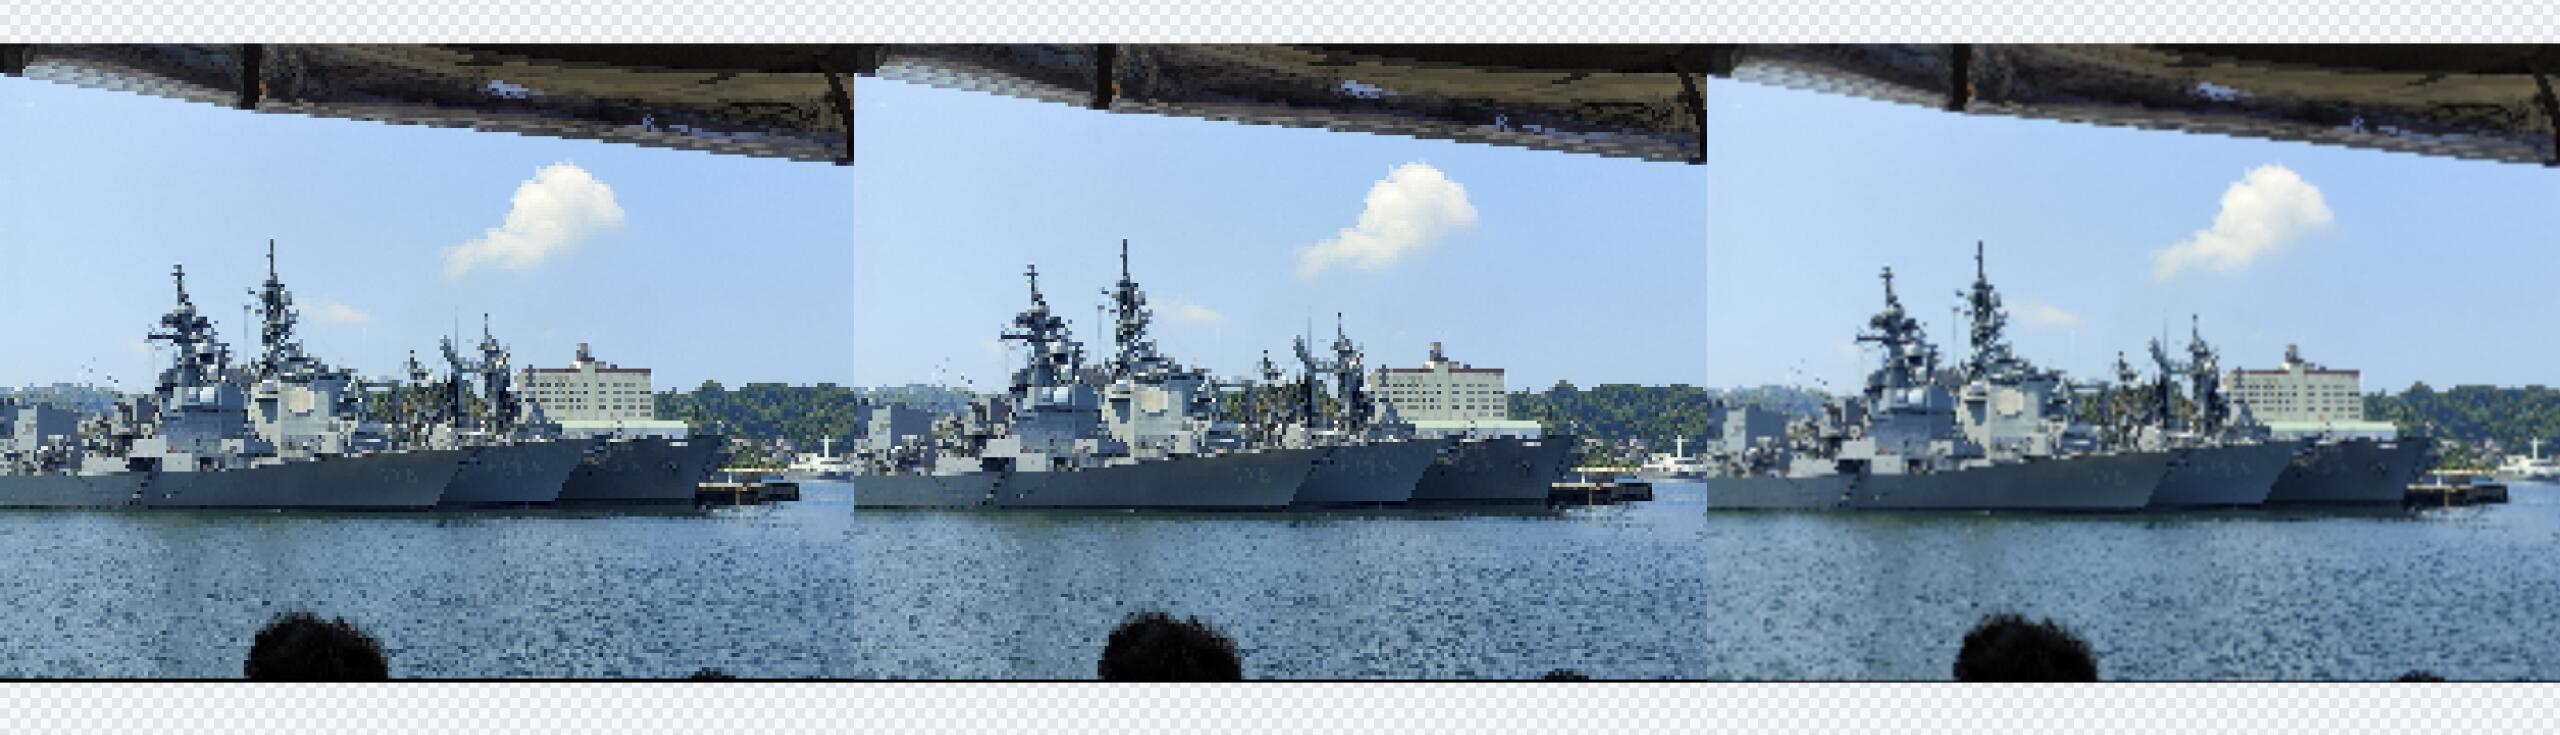
\includegraphics[width=0.8\linewidth]{DemoUp.jpg}
    \caption{Upscaled Image}
    \label{pic:Demo_2}
\end{figure}
\begin{figure}[H]
    \centering
    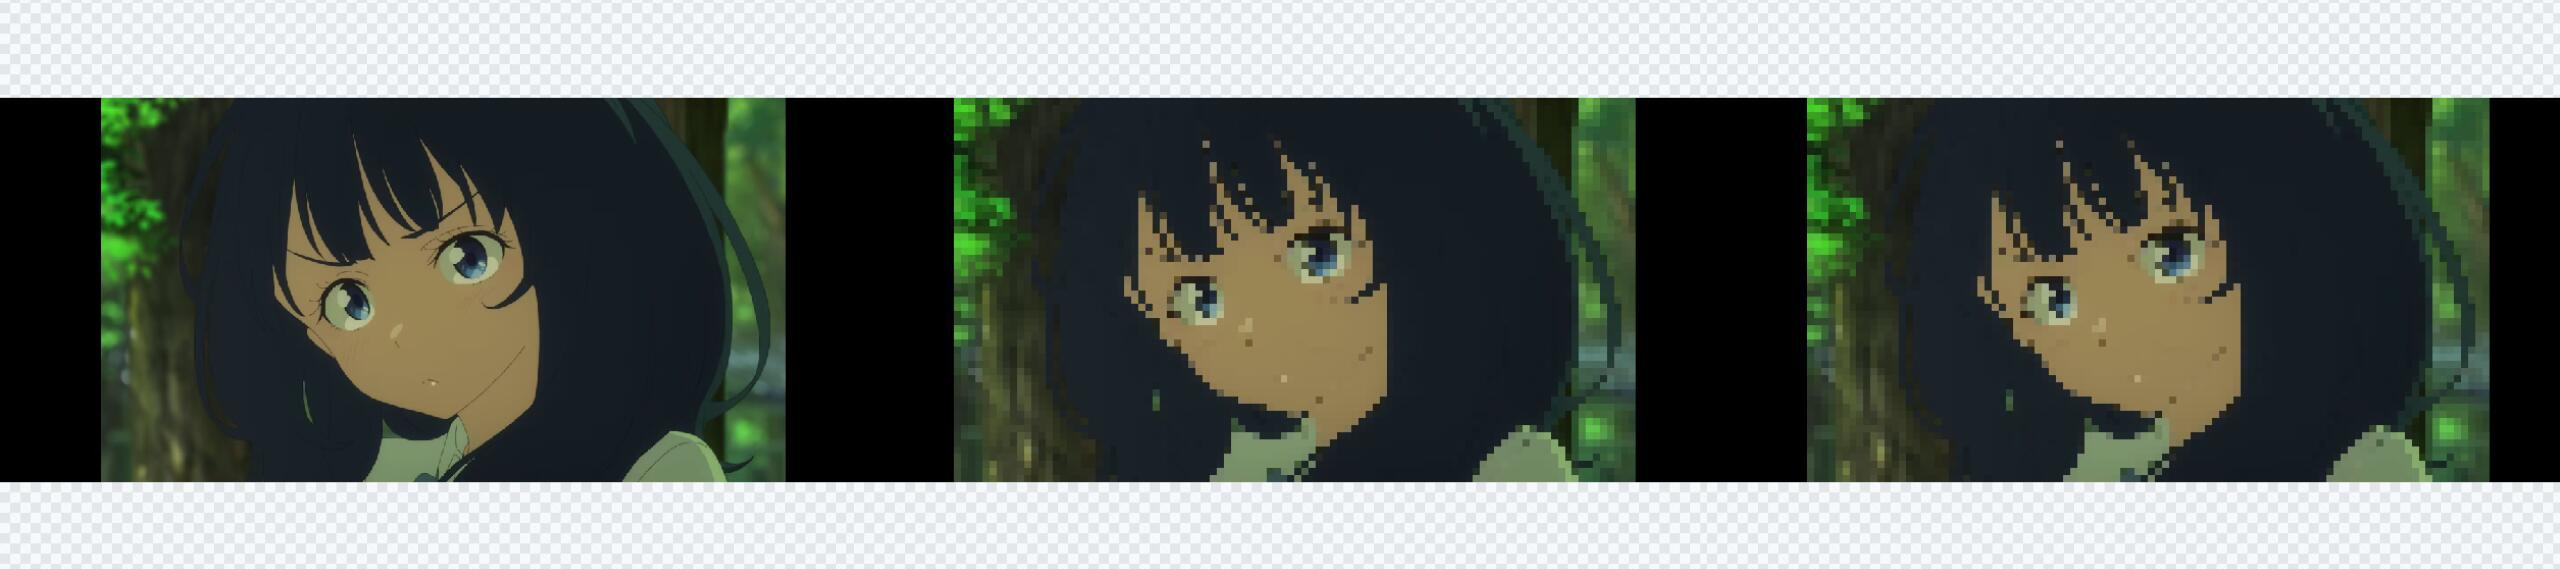
\includegraphics[width=0.8\linewidth]{DemoDown.jpg}
    \caption{Downscaled Image}
    \label{pic:Demo_3}
\end{figure}

From the result, we can see when scaling down the image (\texttt{scale} < 1), both methods provides a similar result. But when scaling up the image (\texttt{scale} > 1), the bilinear interpolation method provides a smoother image than the nearest-neighbor method.\\

\begin{figure}[H]
    \centering
    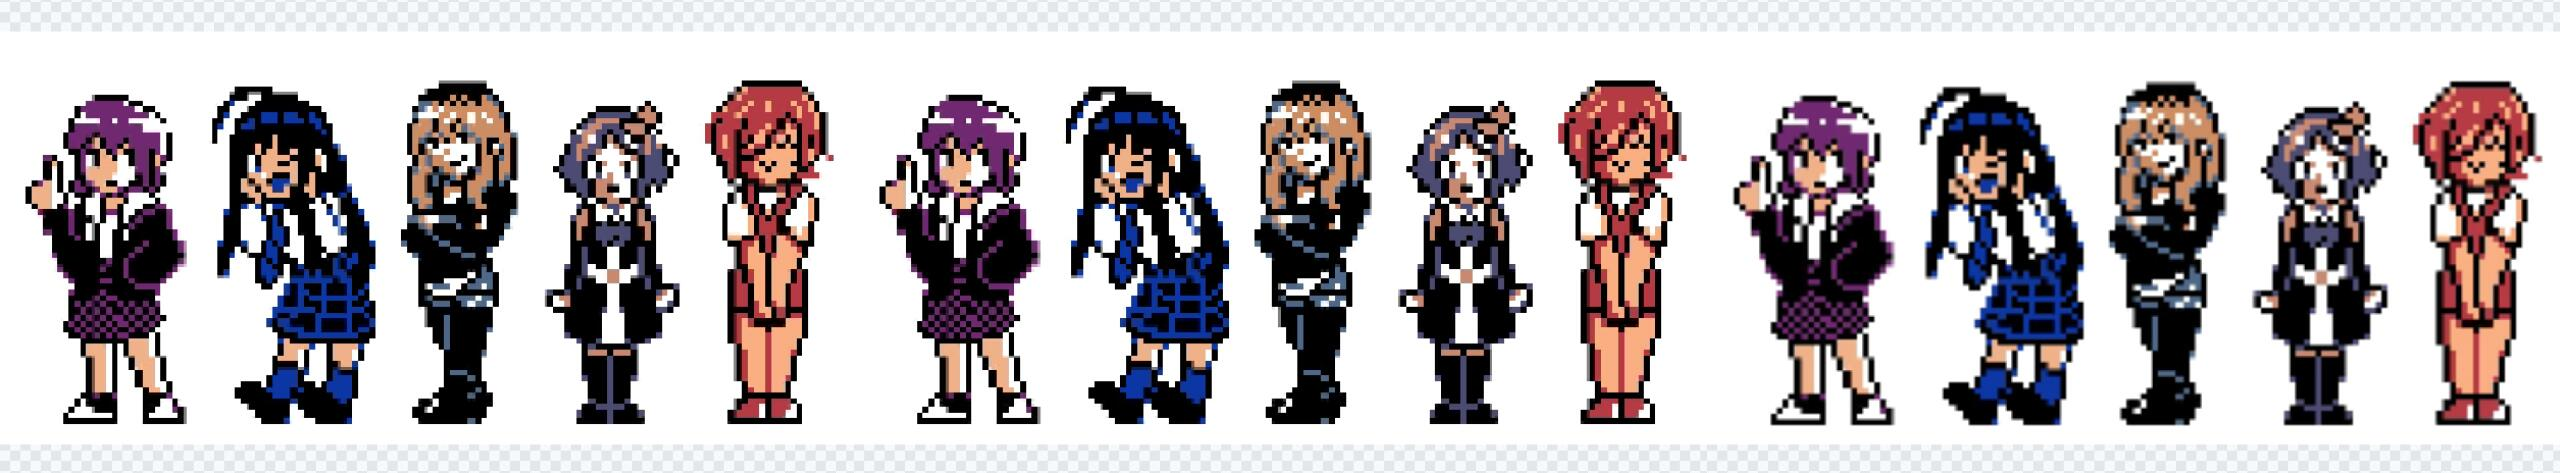
\includegraphics[width=0.8\linewidth]{DemoPixel.jpg}
    \caption{Upscaled Pixel Art Image}
    \label{pic:Demo_3}
\end{figure}

This didn't mean the bilinear interpolation method is better than the nearest-neighbor method. As the following examples in image \ref{pic:Demo_3} shows the bilinear interpolation will screw the pixel art image when scaling up the image. (Demo3: Left: original image, middle, nearest neighbor right: bilinear.)\\


\section{Conclusion}
The experiment successfully implemented a MATLAB image scaling function, $Scaling_K$, capable of performing image resizing using two interpolation methods: nearest-neighbor and bilinear. The implementation addressed critical challenges such as edge handling and coordinate mapping through innovative techniques like adding 0.5 to coordinates and using floor rounding. By comparing the two interpolation methods, we discovered that nearest-neighbor interpolation preserves pixel art better, while bilinear interpolation provides smoother results for photographic images. The research demonstrated that image scaling is nuanced, requiring careful consideration of the image type and desired output quality. Future work could explore more advanced scaling techniques.

\section{References}
No references were used in this experiment.
\end{document}